\chapter{Perspective \& Future Directions}

In chapters \ref{chapter:processor_characterization} and \ref{chapter:grover_algorithm} we demonstrated a universal two-qubit gate on our quantum processor and used it to realize the two-qubit Grover search algorithm, achieving probabilistic quantum speed-up. However, this approach to quantum computing cannot be scaled beyond a few qubits, wich is mostly due to the nature of the qubit-qubit coupling that has been chosen: The direct capacitive coupling produces a qubit-qubit interaction which is always on and whose amplitude decreases as $g_{qq}/\Delta_{qq}$. To be able to realize gate times which are shorter than the typical coherence time of Transmon qubits (typically $T_1,T_\phi \simeq\ 1-10 \;\mathrm{\mu s}$) we require coupling strengts $g_{qq}/2\pi \ge 10\;\mathrm{MHz}$. Therefore, in order to switch of spurious coupling between any two qubits below the 5 \% level, a detuning of $\Delta_{qq}\ge 20g \simeq 200\;\mathrm{MHz}$. For a processor where one would couple a large number of qubits using this scheme, the required qubit-qubit detunings would quickly lead to so-called {\it frequency crowding}, i.e. a shortage of available working point frequencies for the different qubits of the processor.

\smallskip

Hence, for a larger-scale quantum processor, it is essential to devise a coupling scheme which allows to deterministically turn on and off the coupling between arbitary qubits. In the literature, several architectures have been proposed for this, using e.g. a parametric coupling between qubits \citep{bertet_parametric_2006} or relying on the storage of quantum information stored in the qubits in a seperate entity, such as a superconducting resonator \citep{galiautdinov_resonatorzero-qubit_2012,mariantoni_implementing_2011}.

\smallskip

In the following section, we will propose a different approach to scalable quantum computing, based on a recently introduced double Transmon qubit \citep{srinivasan_tunable_2011} and using a fixed-frequency, microwave-tunable qubit-qubit coupling scheme as well as a single-shot readout method for individual qubits.

\smallskip

After shortly discussing our proposed architecture, we discuss recent developments in superconducting quantum computing and put them in context with our work, indicating possible future research directions.

\section{Designing a Scalable Architecture for Quantum Bits} \label{section:scalable_architecture}

In this section we describe our proposal for a scalable multi-qubit architecture based on superconducting Transmon qubits and fulfilling all of DiVincenzo's criteria for the realization of a quantum computer, as discussed in section \ref{section:divincenzo_criteria}. \citep{steane_how_2007}

\subsection{Requirements}

A scalable architecture for quantum computing should fulfill all criteria discussed above and, in addition do not incur an exponential experimental overhead for each qubit that is added to the quantum computer \citep{blume-kohout_climbing_2002}. Today, the two issues that are not addressed well by current qubit architectures, such as the quantum bus architecture used by many groups today \citep{dicarlo_demonstration_2009,wallraff_strong_2004}, which concern the qubit-qubit coupling and the readout of individual qubits. The quantum bus architecture, for instance, has an always-on coupling scheme between the qubits described by eq. (\ref{eq:cqed_bus_coupling}) which makes it hard to precisely control the coupling between individual qubits if a large number of them is present. Also, the readout of the qubit register is usually performed as a joint readout of the whole qubit register, thereby not allowing the read out of individual qubits.

\subsection{Qubit Parameters}

\begin{SCfigure}[1.0][ht!]
	\centering
	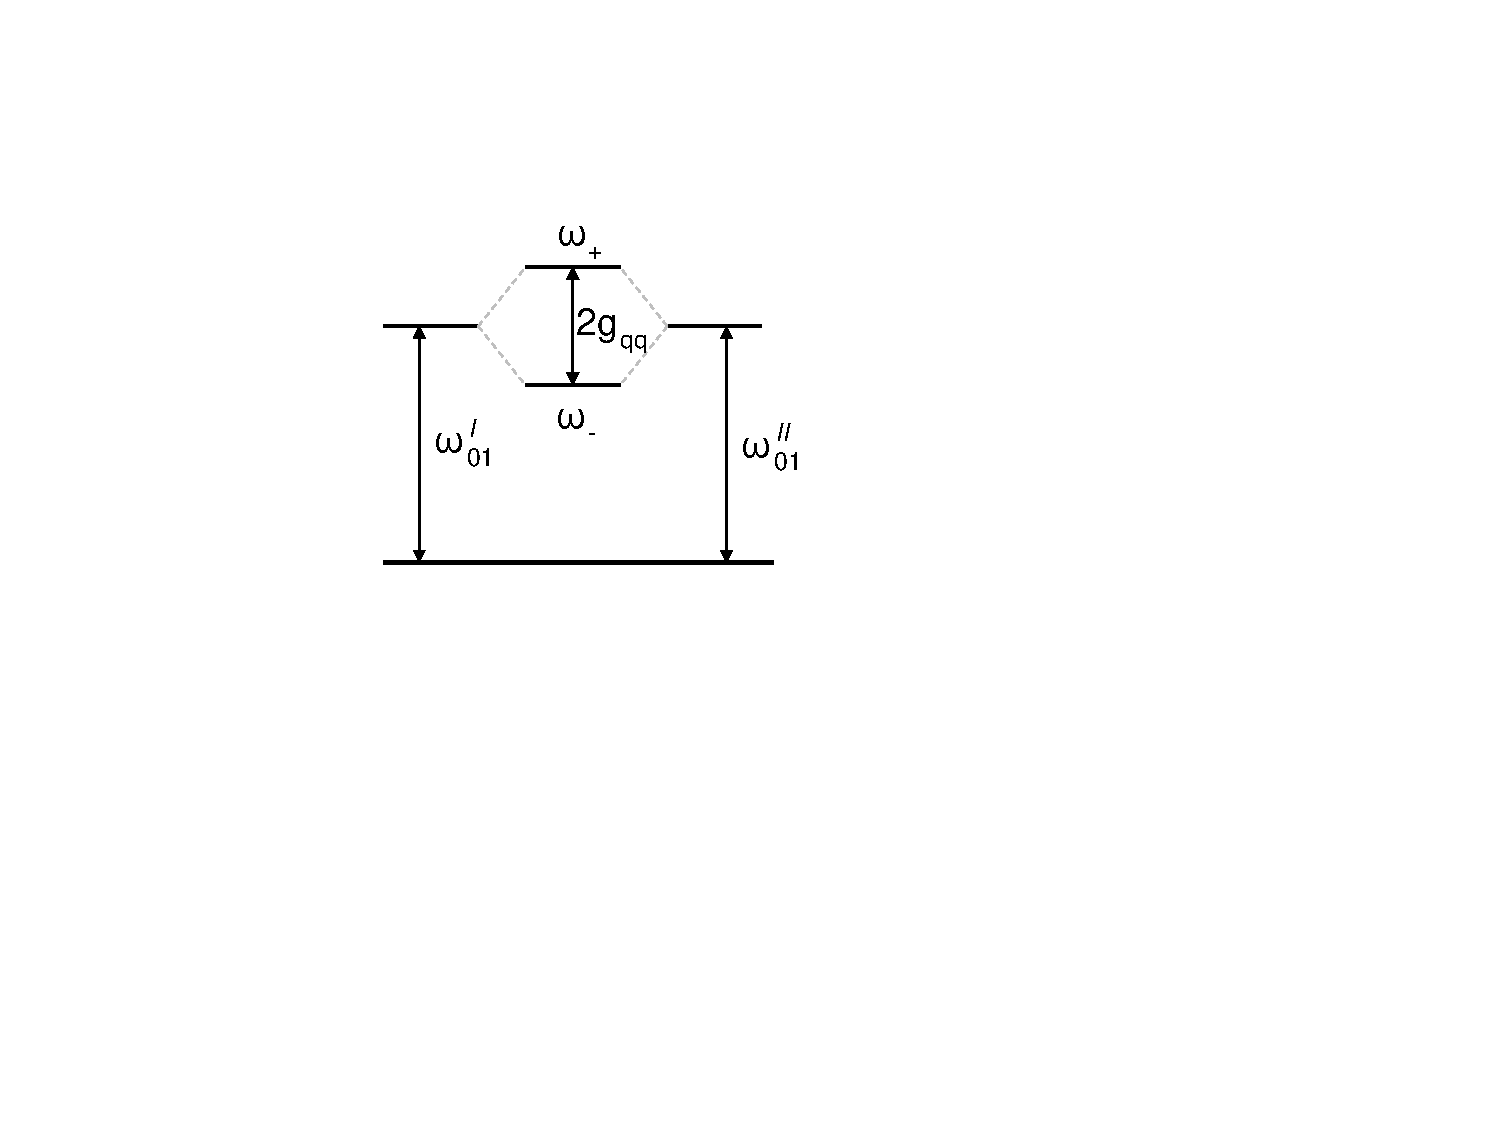
\includegraphics[width=0.35\textwidth]{./material/figures/scalable-architecture/qubit_molecule}
	\caption[...]{...}
	\label{fig:qubit_molecule_energies}
\end{SCfigure}

%
\begin{eqnarray}
\hat{H}_{dt}       & = & \hat{H}_q+\hat{H}_{qq} \\
\hat{H}_{q}/\hbar  & = & \omega_{01}^I\hat{\sigma}_z^I+\omega_{01}^{II}\hat{\sigma}_z^{II} \\
\hat{H}_{qq}/\hbar & = & g_{qq}\left(\hat{\sigma}_+^I\hat{\sigma}_-^{II}+\hat{\sigma}_-^I\hat{\sigma}_+^{II}\right) \\
\end{eqnarray}
%
We can rewrite $\hat{H}_{qq}$ in the eigenbasis $\ket{00}$, $\ket{01}$, $\ket{10}$, $\ket{11}$ of $\hat{H}_q$ as
%
\begin{equation}
\hat{H}_{qq}/\hbar = g_{qq}\left(\ket{10}\bra{01}+\ket{01}\bra{10}\right)
\end{equation}
%
When taking into account the second Transmon level $\ket{2}$, the capacitive coupling induces additional coupling elements
%
\begin{eqnarray}
\hat{H}_{qq}'/\hbar g_{qq} &  = &  \left(\ket{10}\bra{01}+\ket{01}\bra{10}\right) \\
& + & \sqrt{2}\left(\ket{11}\bra{02}+\ket{02}\bra{11}\right) \\
& + & \sqrt{2}\left(\ket{11}\bra{20}+\ket{20}\ket{11}\right) \\
& + & 2\left(\ket{21}\bra{12}+\ket{12}\bra{21}\right)
\end{eqnarray}
%
\subsection{Qubit-Qubit Coupling}

We couple the double Transmon to the resonator as shown in fig. \ref{fig:double_transmon_schematic} such that each of the two Transmons couples to the resonator with the same constant $g_{01}$. The resulting Hamiltonian, in analogy to Hamiltonian (\ref{eq:cqed_bus_coupling}) is
%
\begin{equation}
\hat{H}_{qr}/\hbar = g_{01}^I\left(\hat{\sigma}_+^I\hat{a}+\hat{\sigma}_-^I\hat{a}^\dagger\right)+g_{01}^{II}\left(\hat{\sigma}_+^{II}\hat{a}+\hat{\sigma}_-^{II}\hat{a}^\dagger \right), \label{eq:double_transmon_resonator_coupling}
\end{equation}
%
where, as before, the Hamiltonian of the resonator is given by eq. (\ref{eq:lc_hamiltonian}). As can be seen, the coupling operator between the two qubits and the resonator contains the sums $\hat{\sigma}_+^{I+II}=\hat{\sigma}_+^I+\hat{\sigma}_-^{II}$ and $\hat{\sigma}_-^{I+II}=\hat{\sigma}_-^I+\hat{\sigma}_-^{II}$. The eigenstates of $\hat{H}_{dt}$ at resonance $\omega_{01}^I)\omega_{01}^{II}$ are given as $\ket{00}$,$\ket{11}$, $\ket{\psi_+}=1/\sqrt{2}(\ket{01}+\ket{10})$ and $\ket{\psi_-}=1/\sqrt{2}(\ket{01}-\ket{10})$. Writing the Hamiltonian (\ref{eq:double_transmon_resonator_coupling}) in this eigenbasis yields
%
\begin{equation}
\hat{H}_{qr} = \sqrt{2}g_{01}\left[\left(\ket{11}\bra{\psi_+}+\ket{\psi_+}\bra{00}\right)\hat{a}+\left(\ket{\psi_+}\bra{11}+\ket{00}\bra{\psi_+}\right)\hat{a}^\dagger\right].
\end{equation}
%
As can be seen, the state $\ket{\psi_-}$ does not couple at all to the resonator, whereas the state $\ket{\psi_+}$ couples to it with an enhanced coupling rate $\sqrt{2}g_{01}$. The states $\ket{01}=(\ket{\psi_+}+\ket{\psi_-})/sqrt{2}$ and $\ket{10}=(\ket{\psi_+}-\ket{\psi_-})/\sqrt{2}$ couple to it at the normal rate $g_{01}$. Thus, if we operate the double Transmon at $\omega_{01}^I=\omega_{01}^{II}$ and ``park'' the qubit in the state $\ket{\psi_-}$, we can effectively switch off the coupling to the resonator. As proposed in \citep{srinivasan_tunable_2011}, we can peform an adiabatic passage $\ket{\psi_-}\to\ket{10}$ to switch on the qubit-resonator coupling of two or more qubits and perform a multi-qubit gate. Going back to the parking state $\ket{\psi_-}$ turns off the coupling again.

\subsection{Designing A Four-Qubit Architecture}

\begin{figure}[ht!]
	\centering
	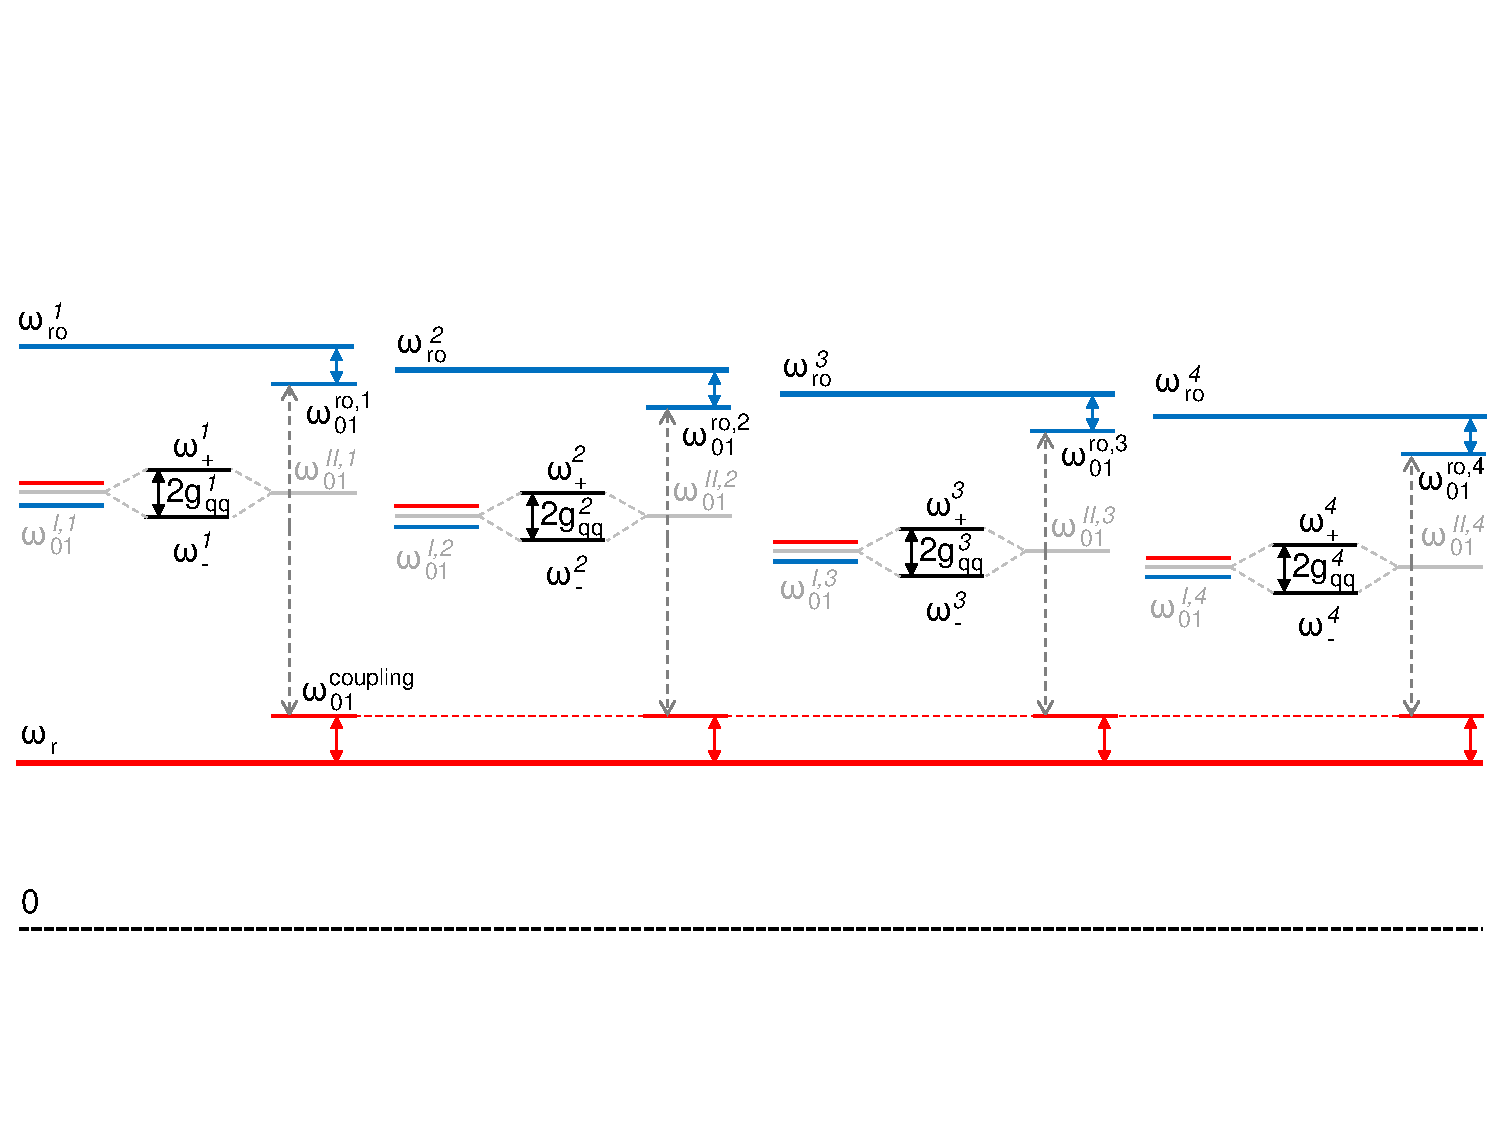
\includegraphics[width=\textwidth]{./material/figures/scalable-architecture/qubit_architecture_energy_levels}
	\caption[]{}
	\label{fig:scalable_architecture_energy_levels}
\end{figure}

\subsection{Implementation}

\begin{figure}[ht!]
	\centering
	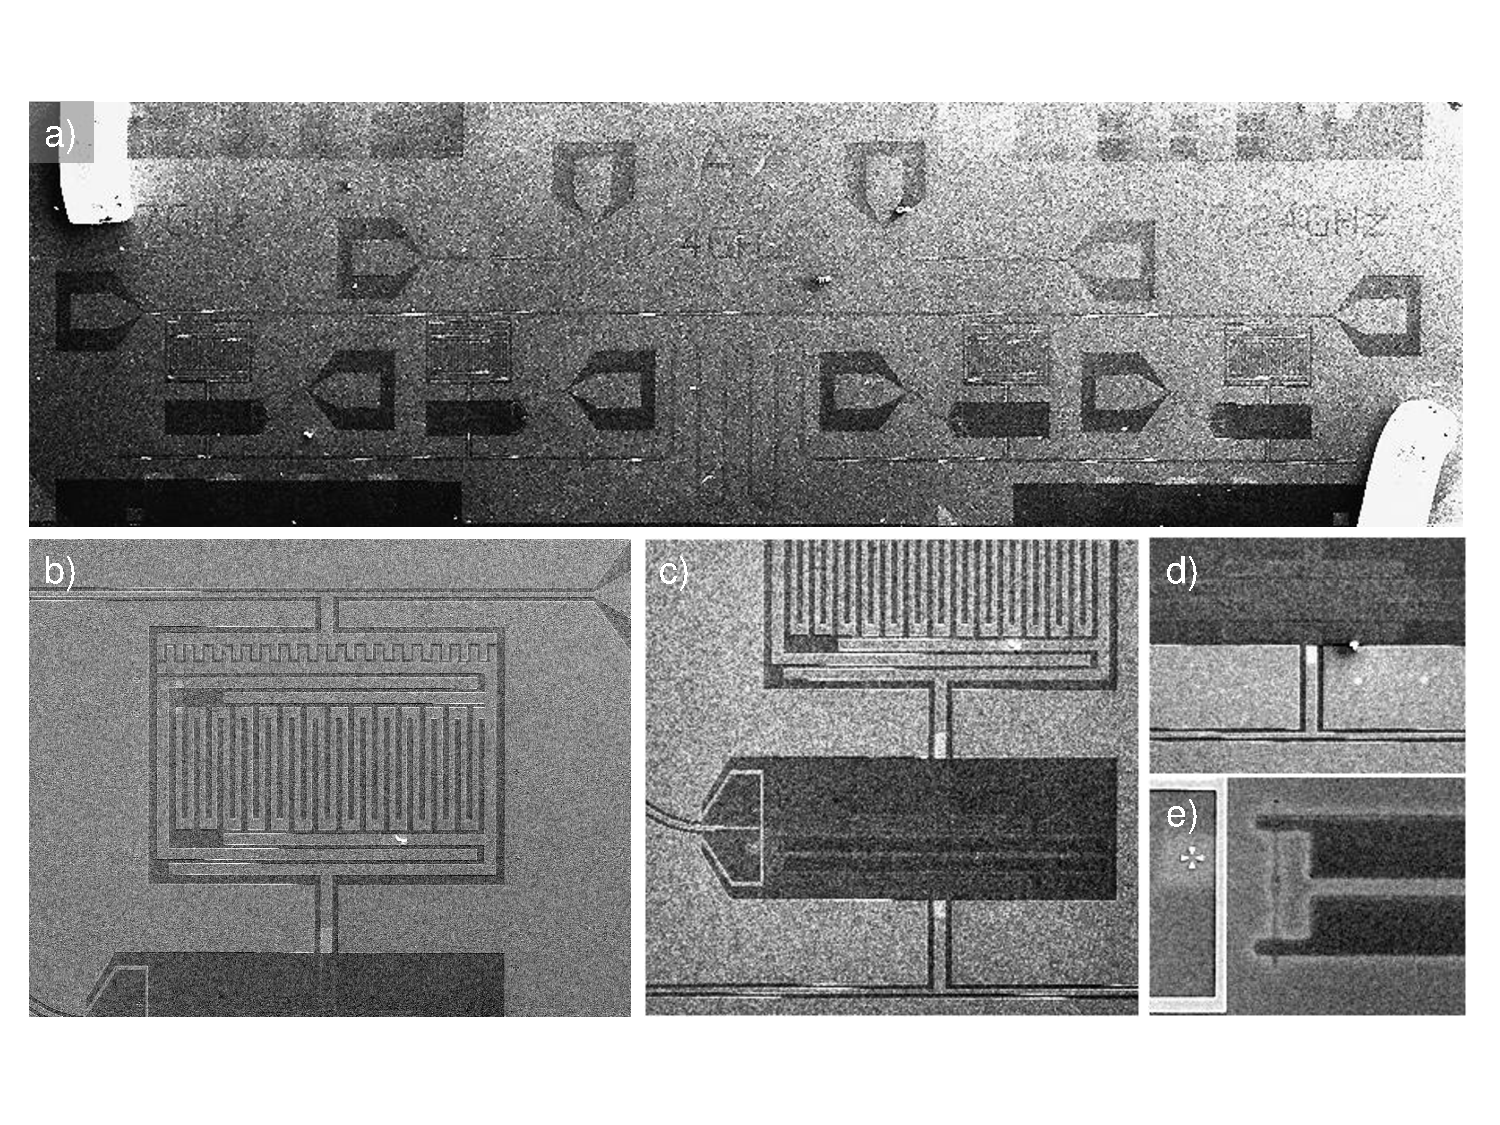
\includegraphics[width=\textwidth]{./material/figures/scalable-architecture/scalable_architecture_photos}
	\caption[]{}
	\label{fig:scalable_architecture_photos}
\end{figure}

\subsection{Scaling Up}

\section{Future Directions in Superconducting QC}

%-Discuss further developments in superconducting qc, such as:

\subsection{3D Circuit Quantum Electrodynamics}

%-Discuss the significance and potential of Q3CED

\subsection{Hybrid Quantum Systems}

%-Discuss hybrid quantum systems such as NV centers and their potential.
%  -Yui's & NTT NV center experiments
%  -Problems and possible solutions

\subsection{Quantum Error Correction \& Feedback}

%-Discuss quantum error correction.
%-Discuss quantum feedback.
%  -Siddiqi experiment, Yale paper
%  -Future directions taking into account the availability of highly coherent Transmon qubits
